\documentclass{article}

\usepackage{graphicx}
\usepackage{tikz}
\usepackage{tikzsymbols}
\usetikzlibrary{calc,patterns,shapes.geometric}
\pagestyle{empty}
\usepackage[margin=0pt]{geometry}
\geometry{papersize={14in,12in}}

\def\centerarc[#1](#2)(#3:#4:#5){\draw[#1] ($(#2)+({#5*cos(#3)},{#5*sin(#3)})$) arc (#3:#4:#5);}

\begin{document}
	\begin{figure}
		\centering
		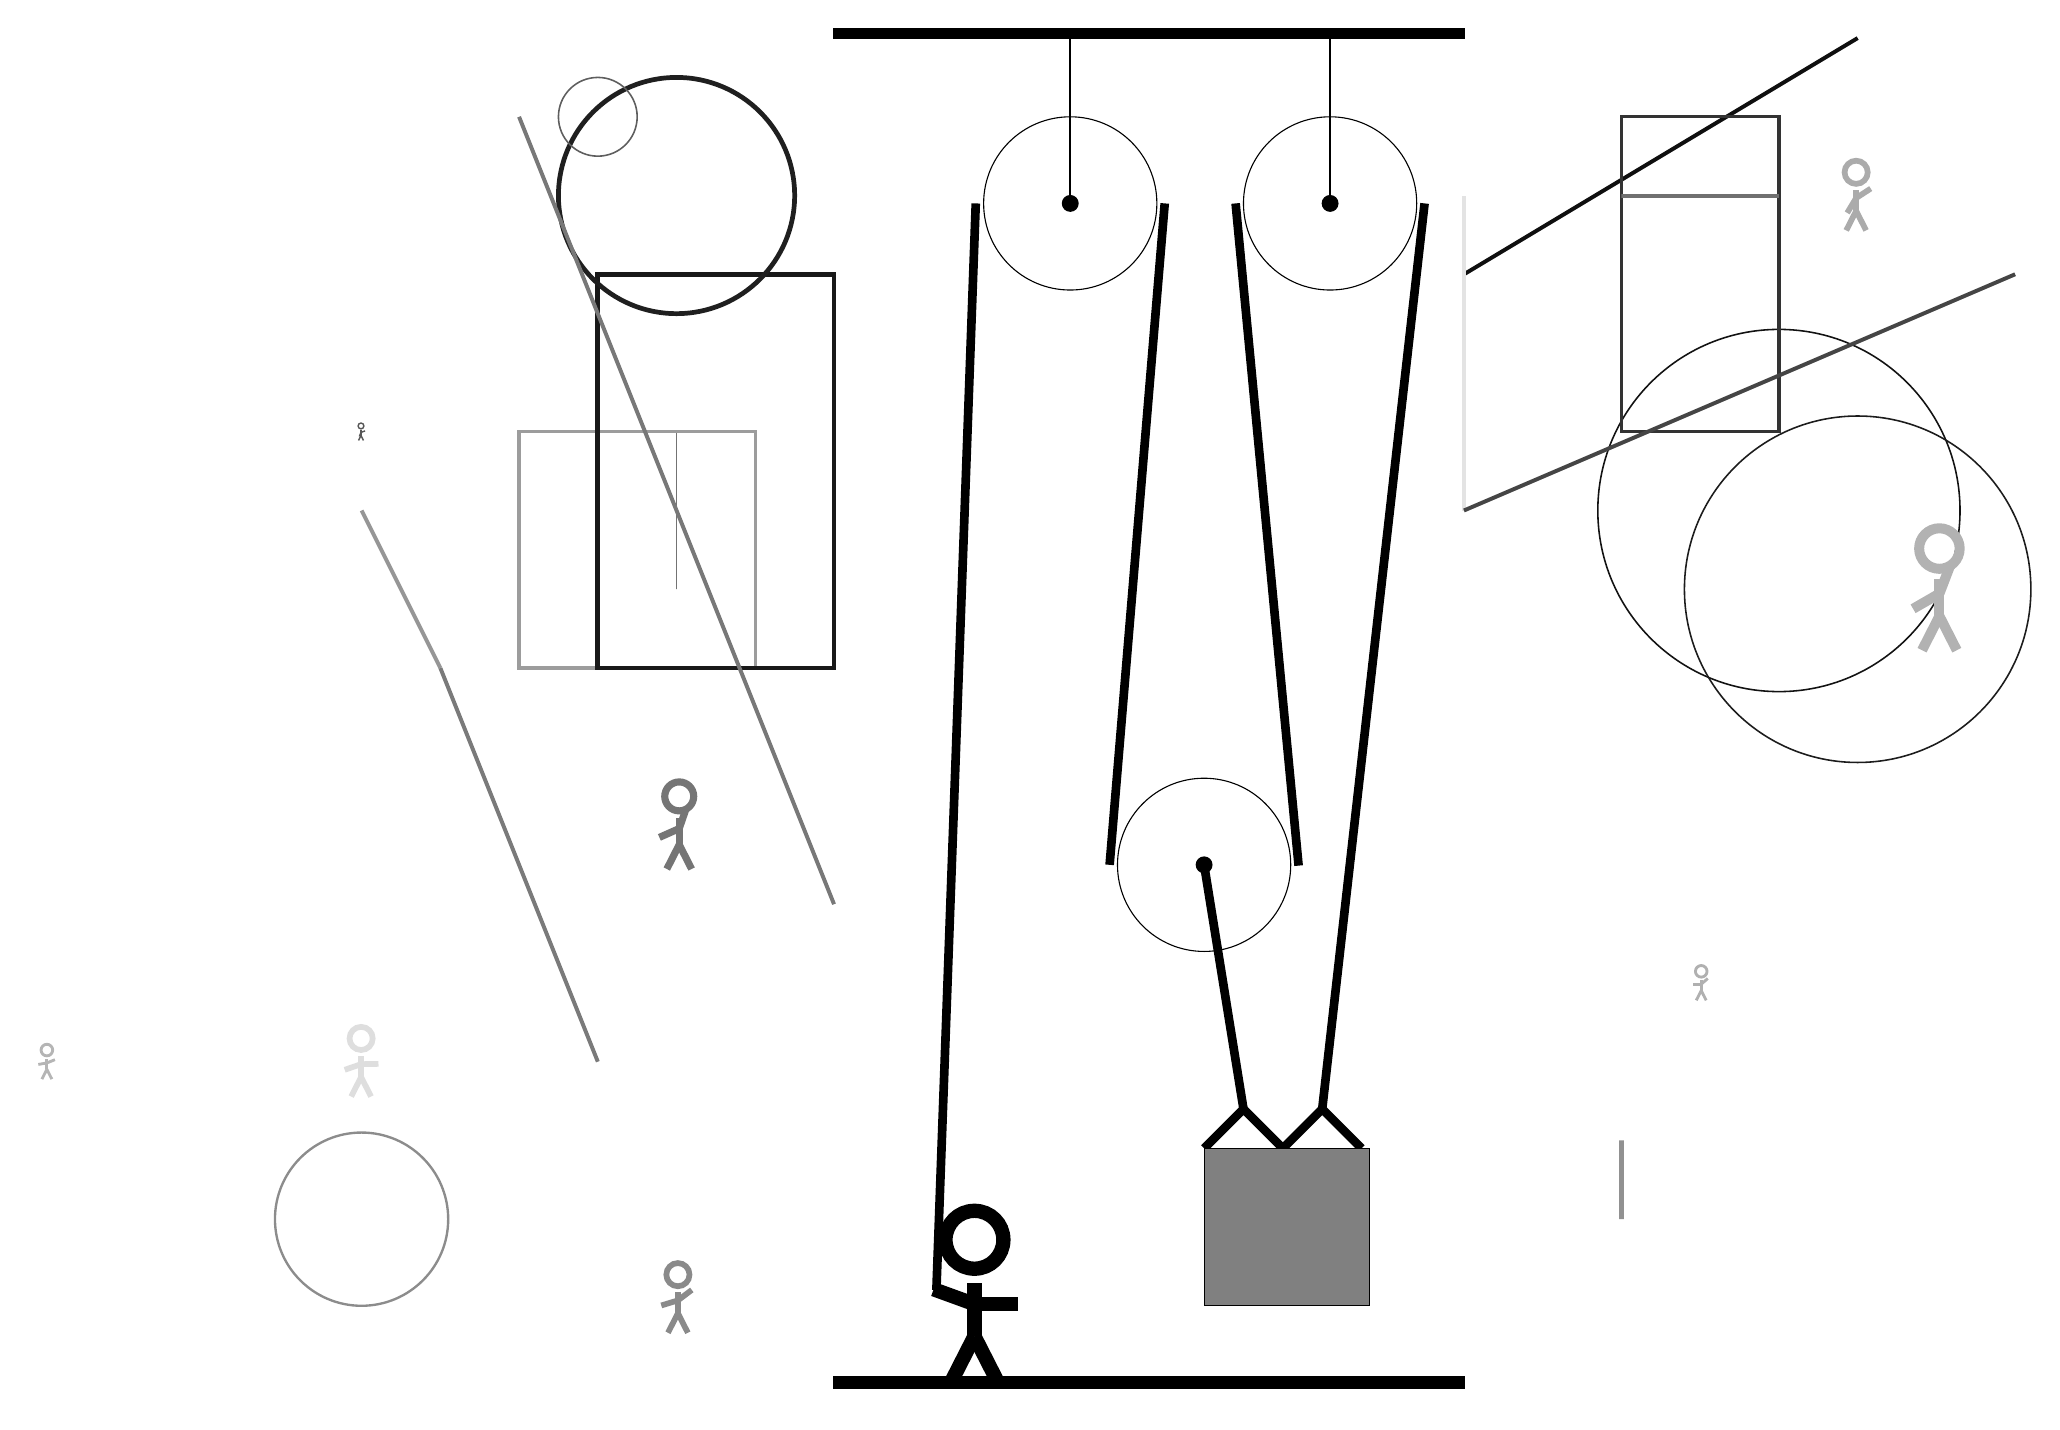
\begin{tikzpicture}
			%%%%% START %%%%%
			
			\draw[fill=black] (-2, 14) rectangle (6, 14.125);
			
			\draw (1, 11.9) circle (1.1);
			\draw[fill=black] (1, 11.9) circle (0.1);
			\draw[thick] (1, 11.9) -- (1, 14);
			
			\draw (4.3, 11.9) circle (1.1);
			\draw[fill=black] (4.3, 11.9) circle (0.1);
			\draw[thick] (4.3, 11.9) -- (4.3, 14);
			
			\draw (2.7, 3.5) circle (1.1);
			\draw[fill=black] (2.7, 3.5) circle (0.1);
			
			\draw[line width=0.2mm, color=black!55] (-4, 9) rectangle (-4, 7);
			
			\draw [line width=0.2mm, color=black!93](10, 8) circle (2.3);
			\draw[line width=0.5mm, color=black!94](6, 11) -- (11, 14);
			\draw[line width=0.4mm, color=black!80] (8, 13) rectangle (10, 9);
			\node[line width=0.2mm, color=black!29] at (-12, 1) {\Strichmaxerl[2][10][22]};
			
			\draw[line width=0.5mm, color=black!52](-7, 6) -- (-5, 1);
			
			\node[line width=0.2mm, color=black!54] at (-4, 4) {\Strichmaxerl[5][24][71]};
			\draw[line width=0.5mm, color=black!56] (8, 12) rectangle (10, 12);
			\node[line width=0.4mm, color=black!31] at (9, 2) {\Strichmaxerl[2][0][41]};
			\draw[line width=0.5mm, color=black!41](-7, 6) -- (-8, 8);
			\node[line width=0.6mm, color=black!46] at (-4, -2) {\Strichmaxerl[4][17][37]};
			
			\draw[line width=0.4mm, color=black!39] (-3, 6) rectangle (-6, 9);
			\draw [line width=0.3mm, color=black!45](-8, -1) circle (1.1);
			
			\draw[line width=0.6mm, color=black!90] (-2, 6) rectangle (-5, 11);
			\draw [line width=0.6mm, color=black!88](-4, 12) circle (1.5);
			\draw[line width=0.6mm, color=black!43] (8, -1) rectangle (8, 0);
			
			\draw [line width=0.2mm, color=black!63](-5, 13) circle (0.5);
			
			\draw[line width=0.5mm, color=black!11](6, 8) -- (6, 12);
			\node[line width=0.5mm, color=black!66] at (-8, 9) {\Strichmaxerl[1][68][20]};
			\node[line width=0.6mm, color=black!13] at (-8, 1) {\Strichmaxerl[4][19][1]};
			\draw[line width=0.5mm, color=black!73](6, 8) -- (13, 11);
			
			\node[line width=0.7mm, color=black!30] at (12, 7) {\Strichmaxerl[7][30][69]};
			\draw [line width=0.2mm, color=black!89](11, 7) circle (2.2);
			\draw[line width=0.5mm, color=black!53](-6, 13) -- (-2, 3);
			\node[line width=0.3mm, color=black!33] at (11, 12) {\Strichmaxerl[4][59][33]};
			
			
			\draw[line width=1.1mm]  (2.7, -0.1) -- (3.2, 0.4) -- (3.7, -0.1) -- (4.2, 0.4) -- (4.7, -0.1);
			\draw[fill=black!50] (2.7, -0.1) rectangle (4.8, -2.1);
			
			\draw[line width=1.1mm](-0.7, -1.9) -- (-0.2, 11.9);
			\centerarc[line width=1.1mm](1, 11.9)(0:180:1.2000000000000002);
			\draw[line width=1.1mm](2.2, 11.9) -- (1.5, 3.5);
			\centerarc[line width=1.1mm](2.7, 3.5)(180:370:1.2000000000000002);
			\draw[line width=1.1mm] (3.9, 3.49) -- (3.1, 11.9);
			\centerarc[line width=1.1mm](4.3, 11.9)(0:180:1.2000000000000002);
			\draw[line width=1.1mm](4.2, 0.4) -- (5.5, 11.9);
			\draw[line width=1.1mm] (3.2, 0.4) -- (2.7, 3.5);
			
			\node at (-0.2, -2) {\Strichmaxerl[10][-20][0]};
			
			\draw[fill=black] (-2, -3) rectangle (6, -3.15);
			
			%%%%% END %%%%%
		\end{tikzpicture}
	\end{figure}	
\end{document}